\documentclass[../../main.tex]{subfiles}

\graphicspath{{../../fig/}}
\setcounter{section}{0}

\begin{document}

\chapter{ワイヤーのたわみ量評価系の開発と、自動化手法の確立}
\label{chap:wiresag}
較正に使う直線偏光はワイヤーに沿う形で生成されるため、ワイヤーがたわんでいる部分から生成される光はその偏光角が
ワイヤーに沿う方向からずれて生成される。そのため、ワイヤーのたわみは較正の精度に影響を及ぼし、系統誤差を生む。
\ref{subsec:wg_wiresag}項では過去に行われた評価手法について述べたが、この手法にはいくつかの問題があった。
本章では、初めにこの問題について今一度触れたあと、それを解決するために開発したワイヤーのたわみを評価する系について述べる。
その後、評価系の原理検証を行い、最後に実際にスパースワイヤーグリッドに対して行った評価結果について述べる。

\section{過去の測定手法における問題点と開発目標}
\colortext{blue}{過去の測定手法についてもう一度 review するべきか、
それとも\ref{subsec:wg_wiresag}項をもっと簡素にし、詳細な内容をこちらに持ってくるべきか、
現在のようにrefするだけにするべきか悩んでいる。}

過去の測定手法については\ref{subsec:wg_wiresag}項にて述べたとおりであり、その手法にはいくつかの問題点があった。
一つ目の問題点は、その測定精度が低いことである。これにより、たわみ量の系統誤差への寄与を必要以上に大きくしている疑いがある。
また、図\ref{fig:wiresag_result_old}にて示されているように、全てのワイヤーに対してそのたわみ量は
期待される量からどの程度外れているかを判別できておらず、品質の低いワイヤーを選別できていない。
もう一つの問題点は、その測定手法が人力にて行われており、測定のために労力と時間がかかる点である。
これによりスパースワイヤーグリッドの量産、品質の保証・管理のために繰り返し測定することが困難である。
また、人力での測定はその測定結果に人依存のバイアスを産む可能性がある。

以上の問題点を解決するため、
\begin{enumerate}
    \item ワイヤーのたわみ量を $\order{\SI{10}{\mu m}}$ の精度で評価可能であること
    \item 全てのワイヤーのたわみ量を自動的に評価可能であること
\end{enumerate}
という2点の開発目標をもって新たなワイヤーのたわみ量の評価系を開発した。

\section{評価系の概要と評価原理}
\subsection{評価系の概要}
初めに、作成した評価系の概観を図\ref{fig:wiresag_system}に示す。
基本的な評価原理は\ref{subsec:wg_wiresag}項にて述べた過去の手法と同様であり、
ストレートエッジとワイヤーを同一写真内に映るように撮影することで、ストレートエッジとワイヤー間の距離からワイヤーのたわみを評価する。
より高精度な評価と自動化を実現するため、過去の評価系をもとに以下のような変更を加えた評価系を作成した。
\begin{enumerate}
    \item スパースワイヤーグリッドを鉛直方向に立てて撮影を行う
    \item スパースワイヤーグリッドとカメラをアクチュエータを用いて自動的に動かす
    \item 一つのワイヤーに対して両端と中央だけでなく、複数の点で撮影を行う
\end{enumerate}

アクチュエータによる自動化を容易にするため、スパースワイヤーグリッドを鉛直方向に立てる。
また、詳細は次節にて述べるが、この配置によりたわみの評価精度が向上する。
たわみの測定の基準となるストレートエッジはスパースワイヤーグリッドの目の前 $\SI{5}{mm}$ のところに固定されている。
使用したストレートエッジは過去のものと同じく大西測定株式会社製の 140-1000B であり、このストレートエッジは真直度A級 $\SI{30}{\mu m}$ が保証されている。
自動化の要であるアクチュエータは、スパースワイヤーグリッドを鉛直方向に動かすために Openbuilds 社の V-Slot NEMA 23 Linear Actuator (Belt Driven) を、
カメラを水平方向に動かすために Openbuilds 社の V-Slot NEMA 17 Linear Actuator (Belt Driven) を用いた。
どちらもベルト駆動式であり、ステッピングモーターを用いて位置制御を行うことができる。
スパースワイヤーグリッドに取り付けられたアクチュエータは、ストレートエッジとワイヤーの距離をカメラの画角に収まるように近づけるために使用され、
カメラに取り付けられたアクチュエータは、撮影位置を変え、ストレートエッジとワイヤーの距離を複数の点で測定するために使用される。
アクチュエータの制御には、Galil 社の DMC-4020 というモーションコントローラを用いた。
また、カメラは

\begin{figure}[H]
    \centering
    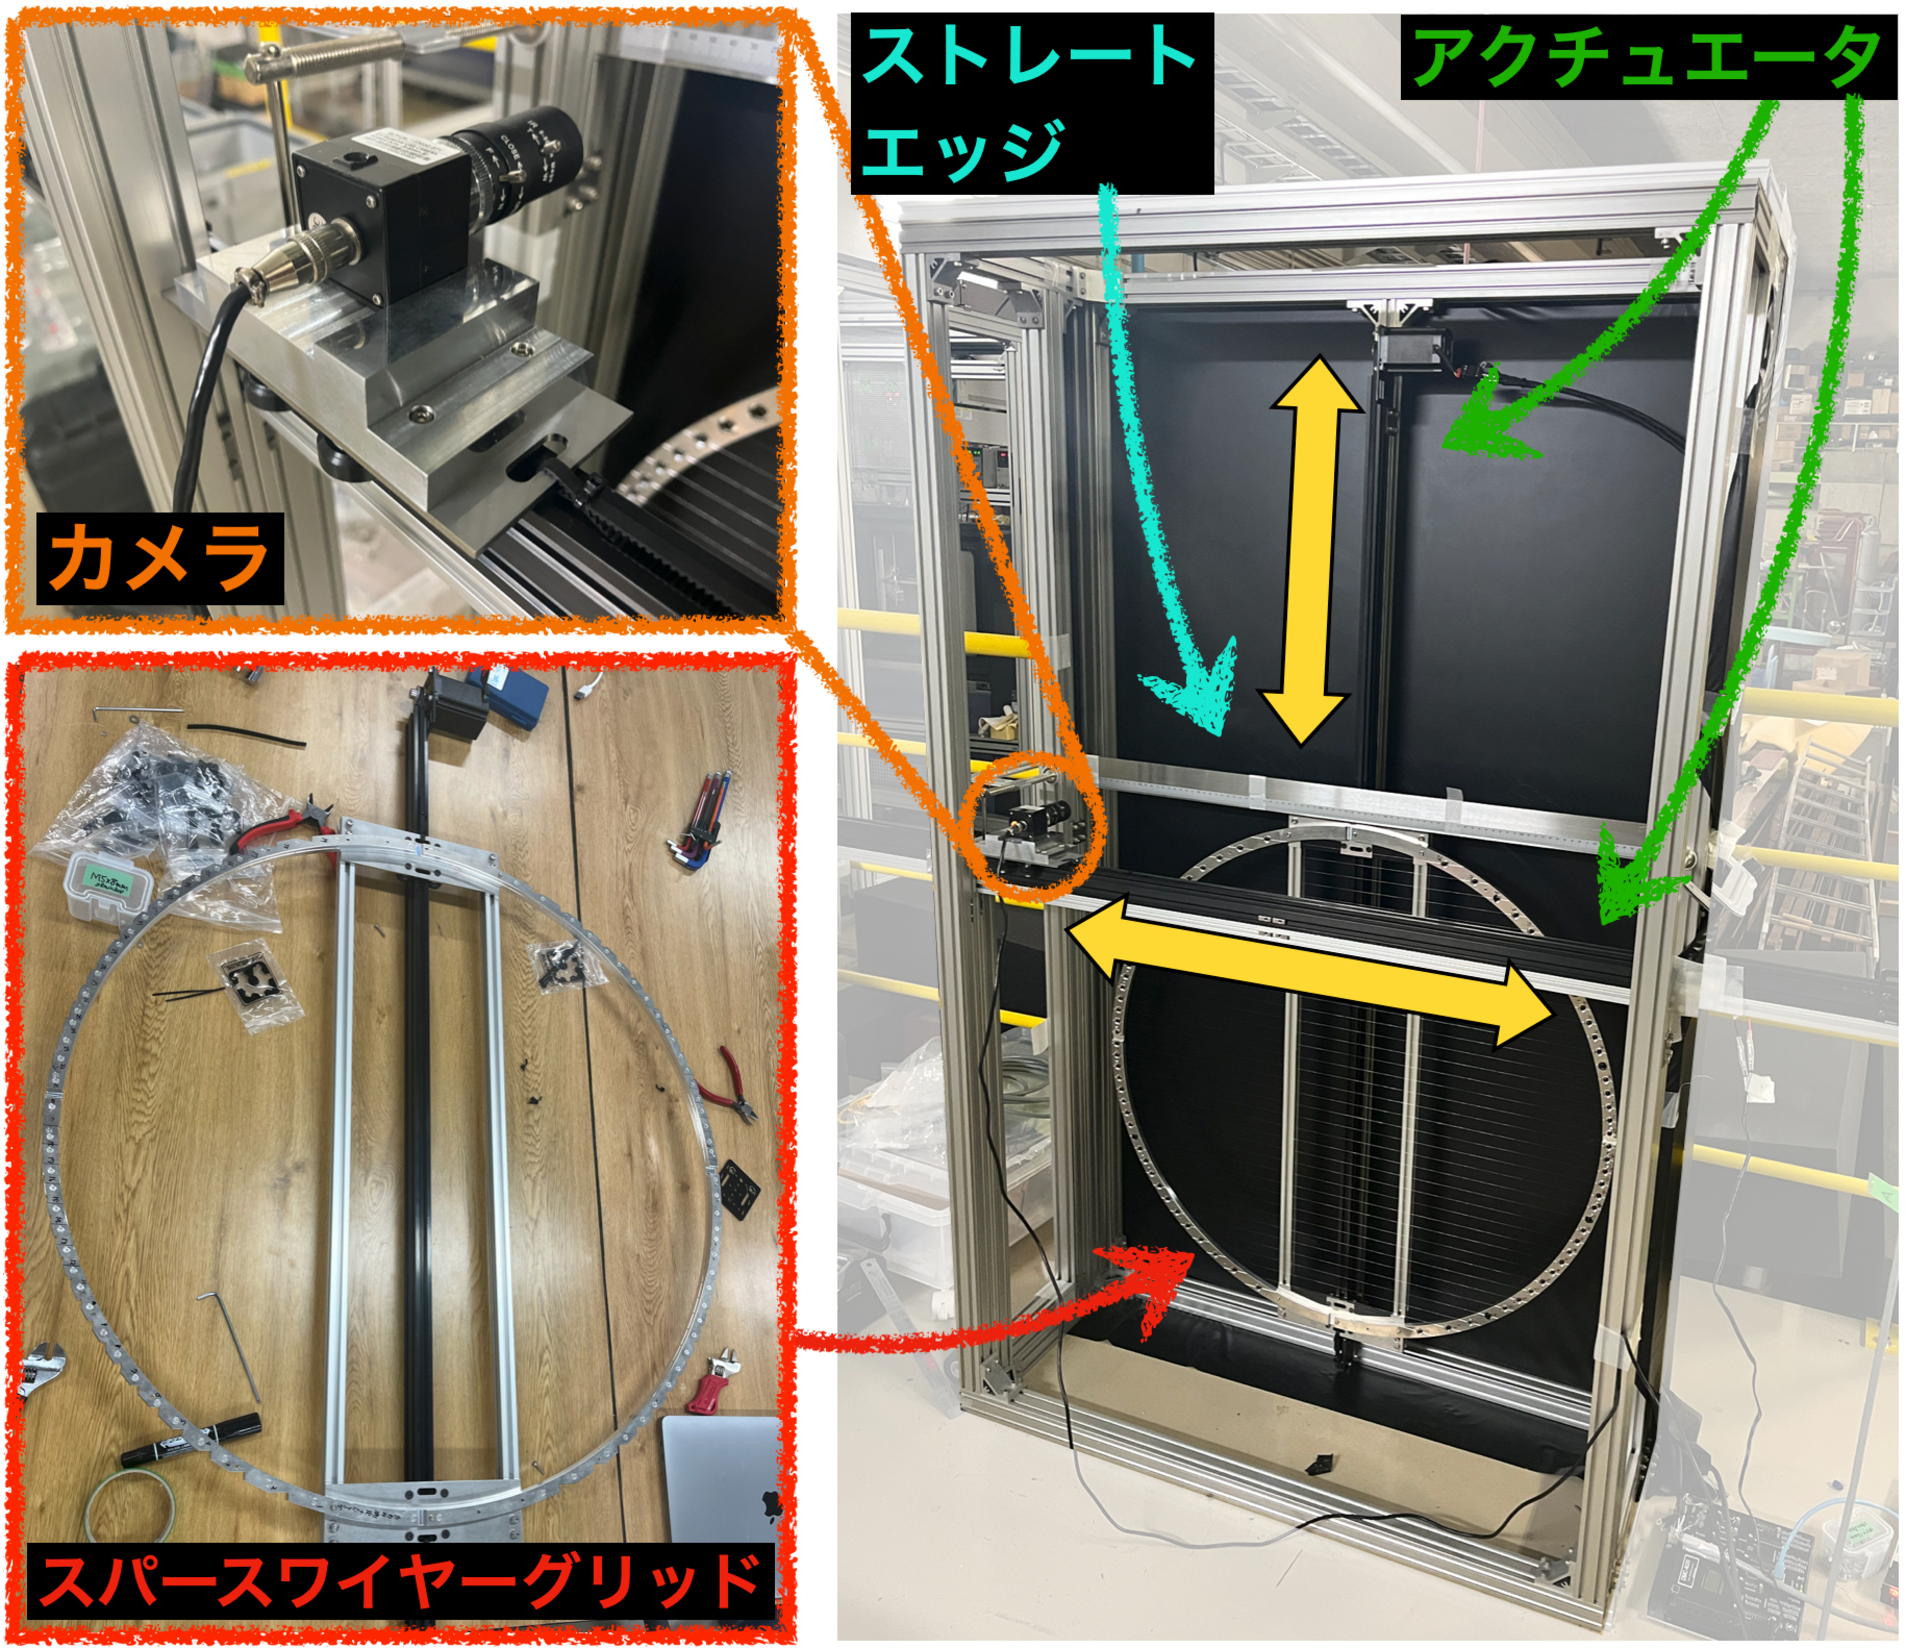
\includegraphics[width=0.8\textwidth]{wiresag/wiresag_system.pdf}
    \caption{ワイヤーのたわみ量評価系の概観}
    \label{fig:wiresag_system}
\end{figure}

\subsection{評価原理}
図\ref{fig:wiresag_concept}に評価原理の概念図を示す。
$x_{0},\,x_{1},\,\cdots,\,x_{n}$ は撮影箇所の位置を表し、$z_{0},\,z_{1},\,\cdots,\,z_{n}$ は各写真から測定されるストレートエッジとワイヤーの距離である。
得られた $x_{i},\,z_{i}$ を横軸 $x$、縦軸 $z$ でプロットすると、ワイヤーの概形を表す曲線が得られる。
ワイヤーの理論曲線はワイヤーの素材、かかっている張力により決まるカテナリー曲線であるため、
得られた曲線をカテナリー曲線で fitting することでワイヤーのたわみ量を評価することができる。

ワイヤーの概形を表すカテナリー曲線は、$T$ をワイヤーにかかる張力、$\rho_{\mathrm{W}}$ をワイヤーの密度、
$R_{\mathrm{W}}$ をワイヤーの半径、$L_{\mathrm{frame}}$ をワイヤーを固定している両端間の距離として
\begin{align}
    \label{eq:wiresag_catenary_nominal}
    f(x;a) &= a\cosh\qty(\dfrac{x+L_{\mathrm{frame}}/2}{a}) - a\cosh\qty(\dfrac{L_{\mathrm{frame}}}{2a}) \\
    a &= \dfrac{T}{\rho_{\mathrm{W}}\cdot\pi R_{\mathrm{W}}^2}
\end{align}
と表される。なお、この式は原点 $(0,\,0)$ と $(L_{\mathrm{frame}},\,0)$ を通る拘束条件を課したカテナリー曲線を表している。
スパースワイヤーグリッドにはタングステン製のワイヤーを使うため、その密度はタングステンの密度 $\rho_{\mathrm{W}}=\SI{19.3}{g/cm^3}$ であり、
ワイヤーの半径は $R_{\mathrm{W}}=\SI{0.1}{mm}$ である。
$L_{\mathrm{frame}}$ はどのワイヤーを評価するかによって異なる。
図\ref{fig:wire_number}のようにスパースワイヤーグリッドに張られたワイヤーに通し番号をつけたとき、
スパースワイヤーグリッドの内径が $\SI{790}{mm}$ であり、ワイヤー間のピッチが $\SI{20}{mm}$ であることから、
$n$ 番目のワイヤーにおける $L_{\mathrm{frame},\,n}$ は
\begin{align}
    L_{\mathrm{frame}, n} = 2\sqrt{395^2-(20\cdot(19-n))^2}\ [\mathrm{mm}] \quad (n=1,2,\cdots,19)
\end{align}
と表される。以下ではワイヤー番号を省略し、単純に $L_{\mathrm{frame}}$ と表す。
$a$ は張力に関わるパラメータであり、ワイヤーが緩んでいることを示す指標となる。
そのため、得られた測定値 ($x_{i},\,z_{i}$) に対して、カテナリー曲線のパラメータ $a$ を fitting parameter として
fitting を行い、best fit により得られた $a$ を用いてワイヤーのたわみ量を算出する。
式\eqref{eq:wiresag_catenary_nominal}より、張られたワイヤーの中心部で生じるたわみ量は
\begin{align}
    \label{eq:wiresag_sag}
    d_{\mathrm{sag}} &= f(L_{\mathrm{frame}}/2;a) \\
                     &= a\qty[1-\cosh\qty(\dfrac{L_{\mathrm{frame}}}{2a})]
\end{align}
であり、たわみ角 $\theta_{\mathrm{sag}}$ は
\begin{align}
    \label{eq:wiresag_sag_angle}
    \theta_{\mathrm{sag}} &= \arctan\qty(\dfrac{d_{\mathrm{sag}}}{L_{\mathrm{frame}}})
\end{align}
となる。

\begin{figure}[H]
    \centering
    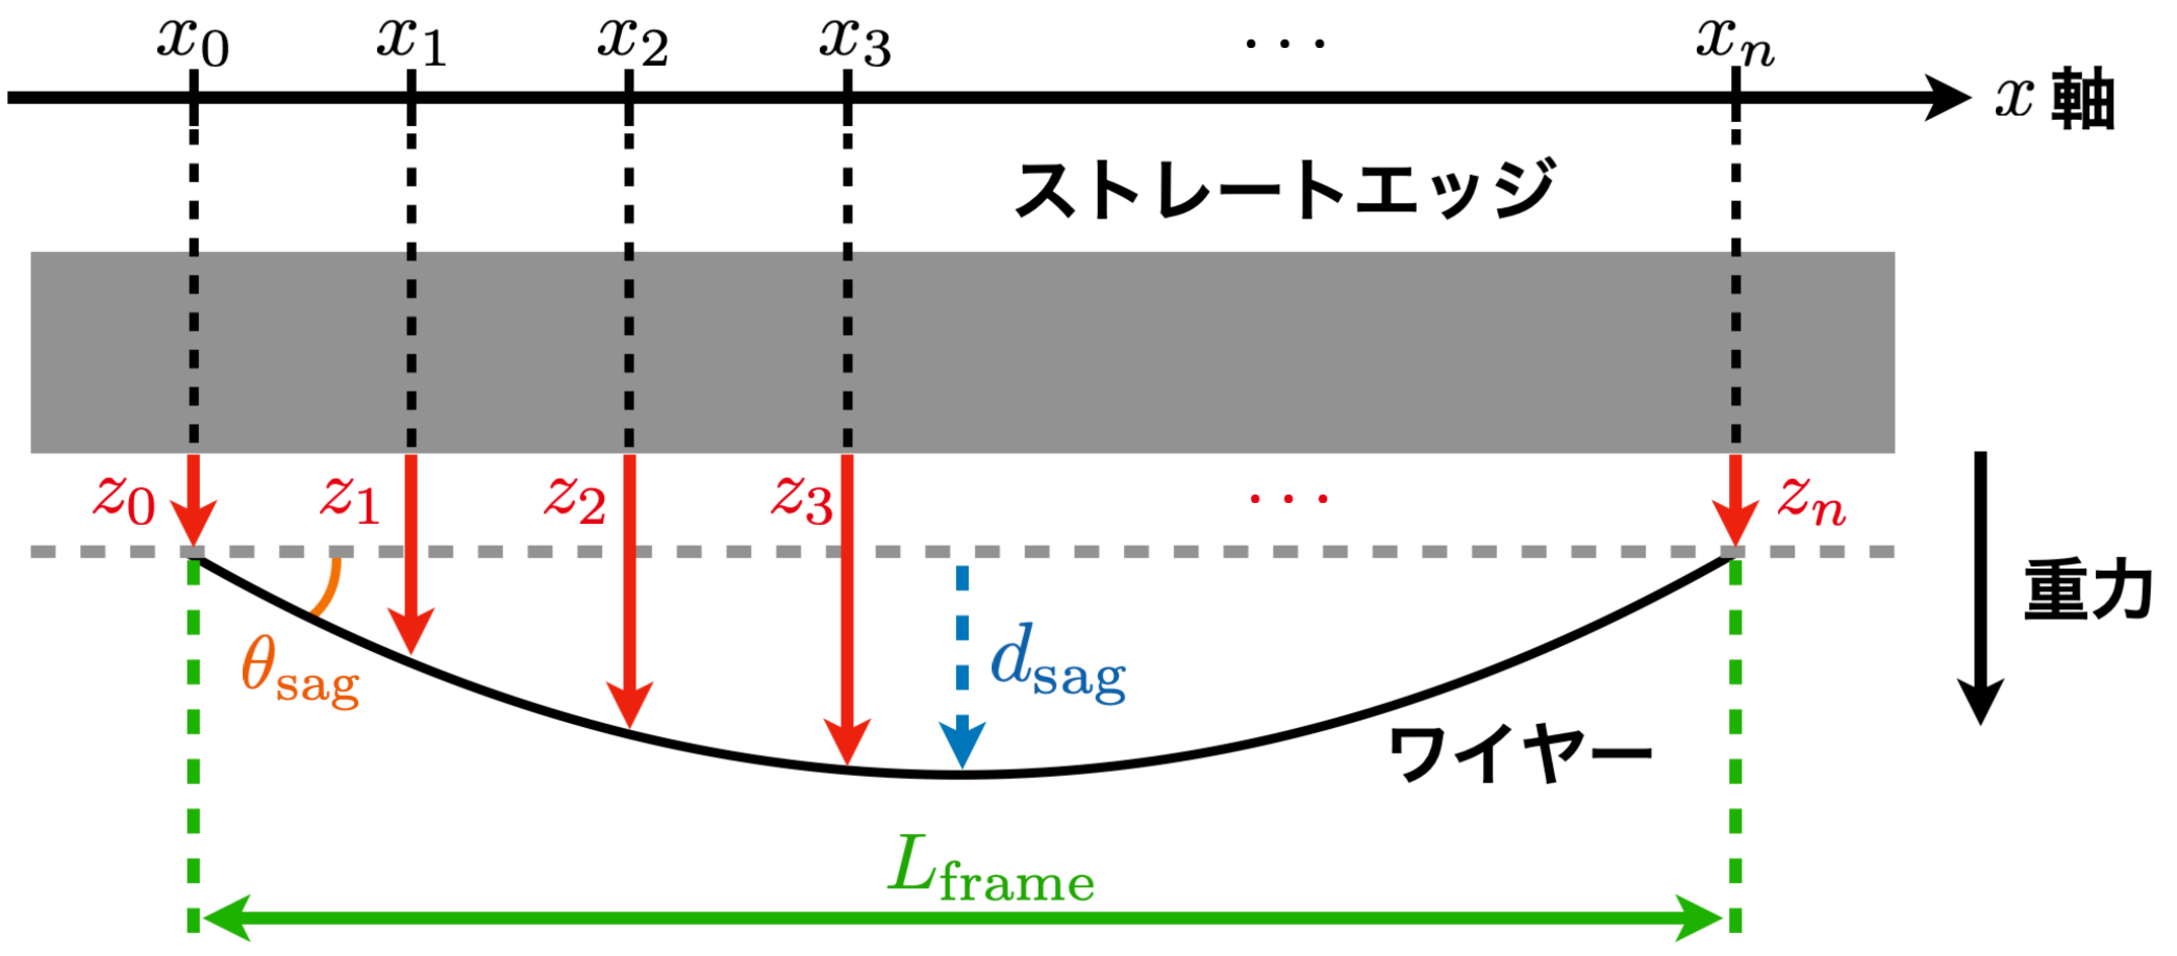
\includegraphics[width=0.8\textwidth]{wiresag/wiresag_concept.pdf}
    \caption{ワイヤーのたわみ量の評価原理}
    \label{fig:wiresag_concept}
\end{figure}
\begin{figure}[H]
    \centering
    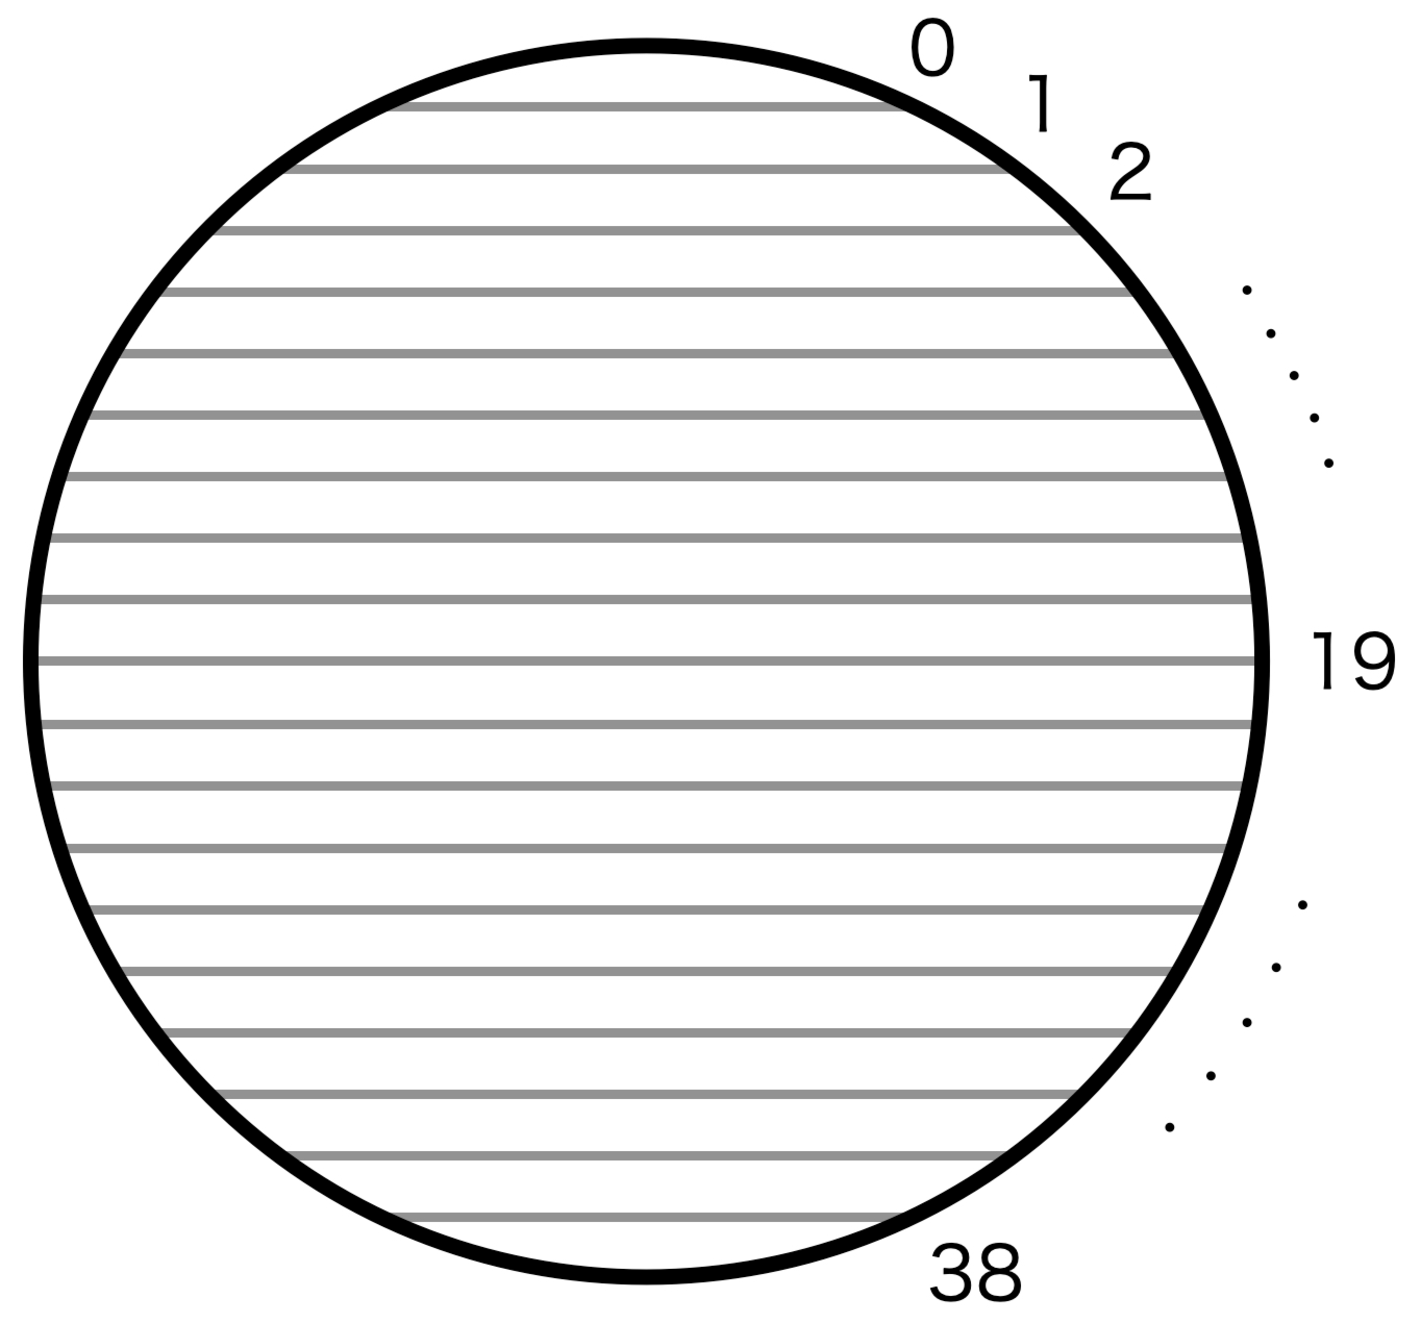
\includegraphics[width=0.5\textwidth]{wiresag/wire_number.pdf}
    \caption{スパースワイヤーグリッドにおけるワイヤー番号}
    \label{fig:wire_number}
\end{figure}

実際の評価系においては、スパースワイヤーグリッド自体が回転し、ワイヤーを固定する両端が水平面上に位置しない場合がある。
図\ref{}のように、ワイヤーの左端が $(0,\,0)$ に位置し、ワイヤーの右端が $(X,\,Y)$ に位置する場合を考える。
このとき、ワイヤーの描くカテナリー曲線は
\begin{align}
    f_{\mathrm{tilt}}(x;a,\,X,\,Y) &= a\cosh\qty(\dfrac{x+c_1}{a}) + c_2 \\
    c_1 &= a\sinh^{-1}\qty[\dfrac{Y}{2a\sinh\qty(\dfrac{X}{2a})}] \\
    c_2 &= -a\cosh\qty(\dfrac{c_1}{a})
\end{align}
となる。ただし、$X,\,Y$ は
\begin{align}
    L_{\mathrm{frame}} &= \sqrt{X^2+Y^2}
\end{align}
を満たす。
測定される $z$ はストレートエッジとワイヤー間の距離であるため、その概形はカテナリー曲線を $-1$ 倍したものであり
\begin{align}
    z_{i} &= -f_{\mathrm{tilt}}(x_{i};a)
\end{align}
として測定値 $(x_{i},\,z_{i})$ に対して fitting を行う。
\begin{figure}[H]
    \centering
    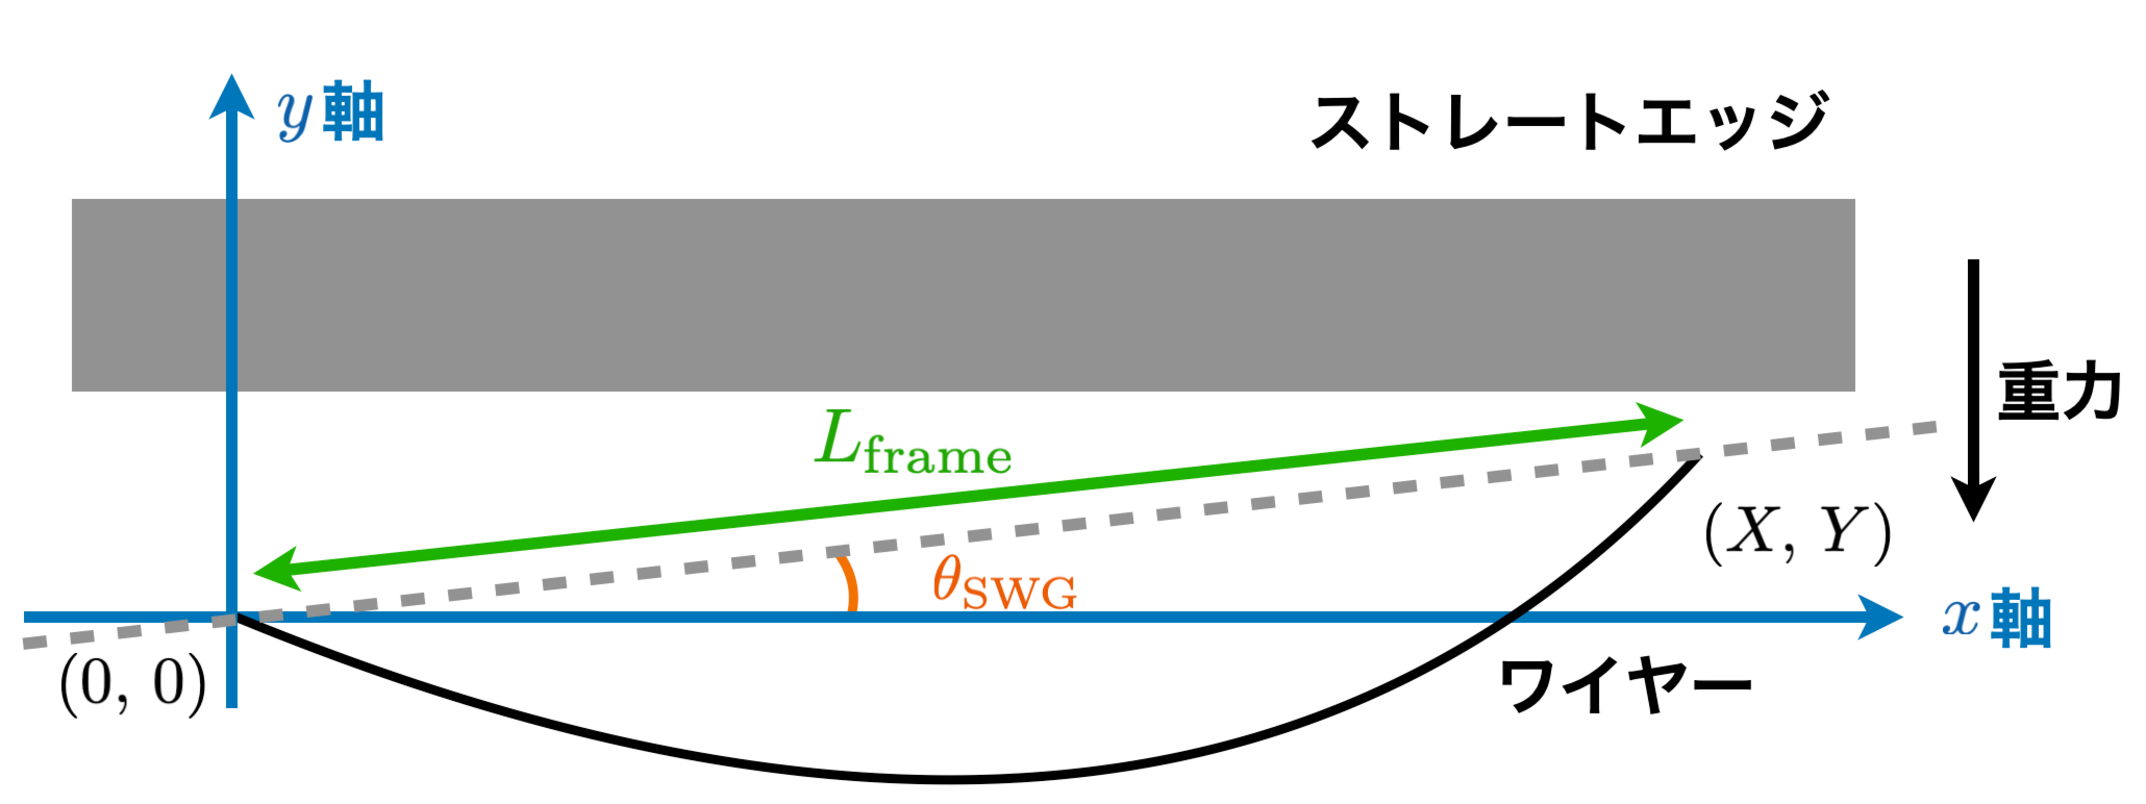
\includegraphics[width=0.8\textwidth]{wiresag/wire_catenary_tilt.pdf}
    \caption{ワイヤーの両端が重力に対して傾いている場合のワイヤーの描くカテナリーの概念図}
    \label{fig:wiresag_concept_tilt}
\end{figure}

図\ref{fig:wiresag_concept_yoko}にワイヤーのたわみ量の評価原理の横から見た概念図を示す。
これは過去の手法における概念図\ref{fig:wiresag_setup_old}を新しい系に合わせて変更したものであり、
カメラから見るとストレートエッジが手前に位置し、ワイヤーがその奥に位置するような配置になっている。
各パラメータの意味とその値、誤差を表\ref{tab:wiresag_concept_yoko_params}に示す。
この系において、測定される量 $z'$ を用いてストレートエッジとワイヤー間の距離 $z$ を表すと、
\begin{align}
    z = \dfrac{z'}{\cos\phi} + \alpha\tan\phi \\
    \phi = \arctan\qty(\dfrac{L_{\mathrm{camera}}}{\beta})
\end{align}
となるが、$L_{\mathrm{camera}}$ は $\SI{0}{mm}$ であるため、
\begin{align}
    z = z'
\end{align}
として問題ない。

\begin{figure}[H]
    \centering
    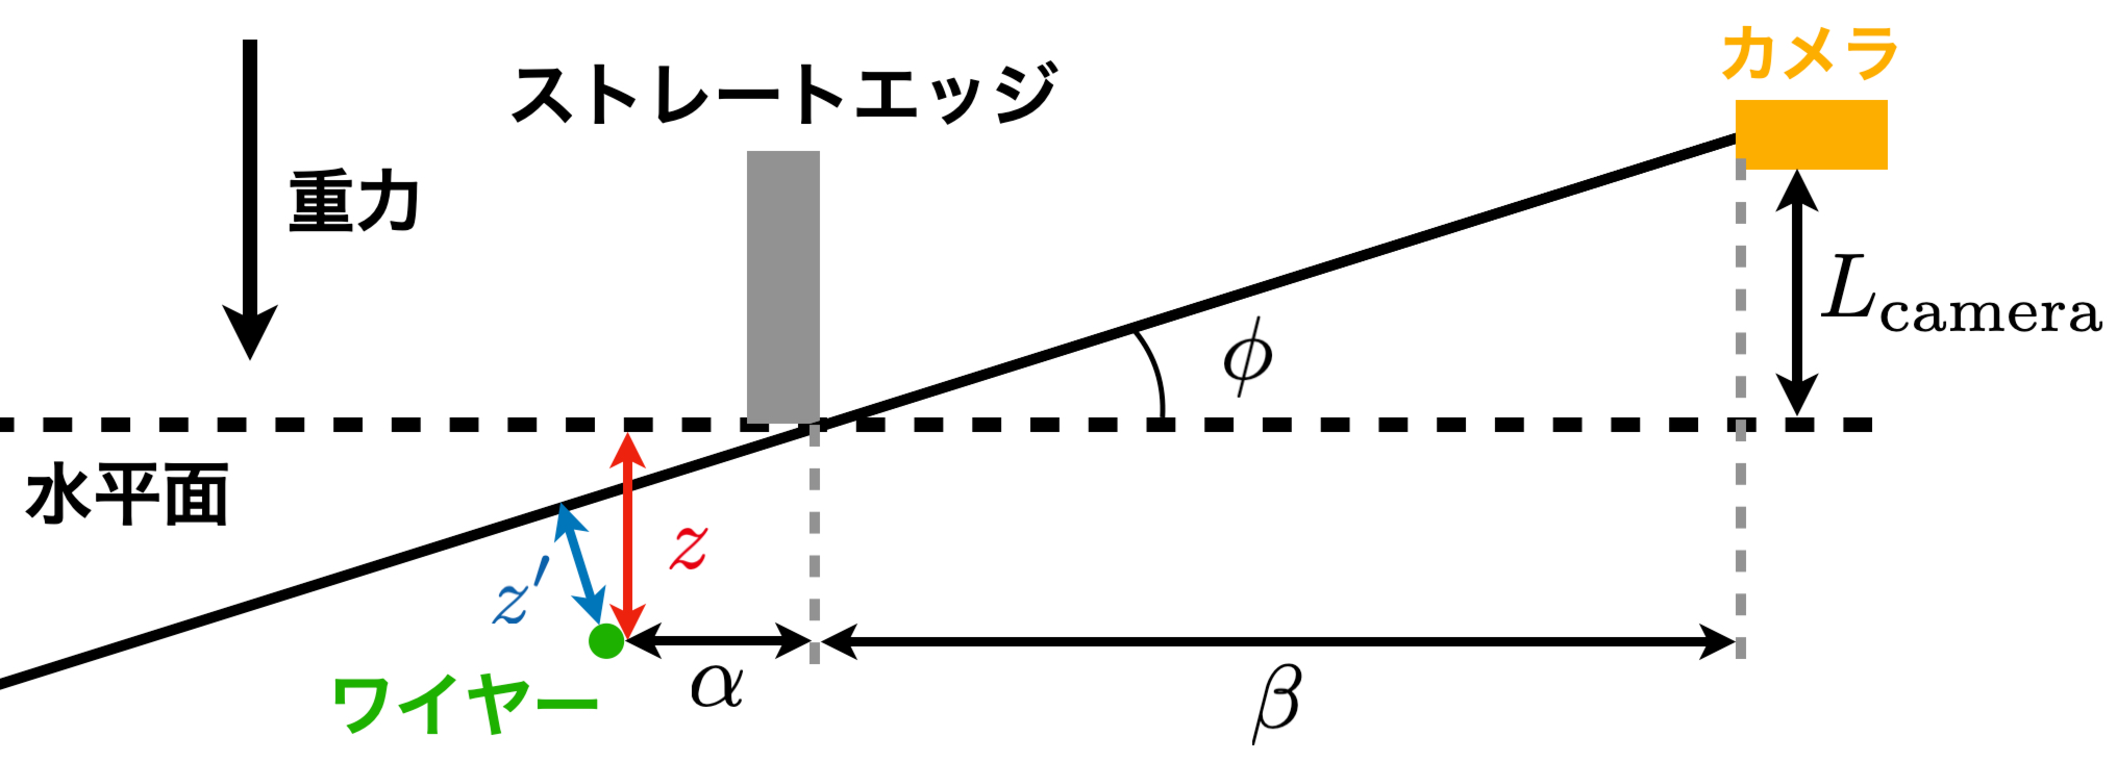
\includegraphics[width=0.8\textwidth]{wiresag/wiresag_concept_yoko.pdf}
    \caption{ワイヤーのたわみ量の評価原理の横から見た概念図}
    \label{fig:wiresag_concept_yoko}
\end{figure}
\begin{table}[H]
    \centering
    \caption{図\ref{fig:wiresag_concept_yoko}における各パラメータの意味と値}
    \begin{tabular}{cccc}
        \hline
        パラメータ & 意味 & 値 & 誤差 \\
        \hline\hline
        $\alpha$ & ストレートエッジとワイヤーまでの水平距離 & $\SI{15}{mm}$ & $\pm\SI{2}{mm}$ \\
        $\beta$ & ストレートエッジからカメラまでの水平距離 & $\SI{205}{\mm}$ & $\pm\SI{5}{mm}$ \\
        $L_{\mathrm{camera}}$ & ストレートエッジ下端の面からカメラまでの鉛直距離 & $\SI{0}{mm}$ & $\pm\SI{0.5}{mm}$ \\
        \hline
    \end{tabular}
    \label{tab:wiresag_concept_yoko_params}
\end{table}

\subsection{評価系の機械設計により生まれる $z$ 誤差の見積もり}
過去の手法においては、$\phi$ が典型的に $5\tcdegree$ 程度と小さくない値であったために、
$L_{\mathrm{camera}}$ や $\alpha$ から $z$ へ大きな誤差が生じていた\cite{swg:murata}。
この誤差を抑えるためには、$\phi$ を小さくすることが重要であるが、
過去の評価系ではスパースワイヤーグリッドを水平面上に設置して撮影しており、
他のワイヤーが撮影対象のワイヤーに重なってしまうため $\phi\sim 0\tcdegree$、すなわち 
$L_{\mathrm{camera}} \sim \SI{0}{mm}$ で撮影することができなかった(図\ref{fig:wiresag_picture_old})。
これを解決するため、スパースワイヤーグリッドを鉛直方向に立てて撮影を行うことで、$L_{\mathrm{camera}}=0\pm\SI{0.5}{mm}$ で撮影を行い、誤差の低減を図った。
新しい評価系において、$z$ の誤差は
\begin{align}
    \delta z = \sqrt{\qty(\dfrac{1}{\cos\phi})^2\delta z'^2 + \qty(\dfrac{\tan\phi}{\cos\phi}+\dfrac{\beta}{\cos^2\phi})^2\delta\phi^2 + \tan^2\phi\delta\beta^2}
\end{align}
と表され、表\ref{tab:wiresag_concept_yoko_params}に示したパラメータの誤差を代入すると、
\begin{equation}
    \delta z \sim \SI{39}{\mu m}
\end{equation}
となる。$z'$ の誤差についてはカメラの $\SI{1}{pixel}$ が対応する長さであり、
次節の解析にて明らかになるがこれは典型的に $5\sim\SI{6}{\mu m}$ 程度である。
また、$z$ にはストレートエッジの真直度由来の誤差 $\SI{30}{\mu m}$ が含まれるため、これも考慮に入れると $z$ の誤差は
\begin{equation}
    \delta z = \sqrt{39^2+30^2}\ \mu\mathrm{m} = \SI{49}{\mu m}
\end{equation}
程度だと見積もられる。

\section{解析手法}
\subsection{解析の流れ}
図\ref{}に実際に撮影された写真の一例を示す。
画像の解像度は $\SI{3264}{pixel}\times\SI{2448}{pixel}$ である。
画像の横軸を $x_{\mathrm{pix}}$、縦軸を $y_{\mathrm{pix}}$ とし、画像の左上を原点 $(0,\,0)$ とする。
また、画像の出力フォーマットは yuyv であり、これは各pixelの輝度に関する情報を失うことなく保存される。
ストレートエッジとワイヤー間の距離 $z$ を算出し、たわみ量を評価するため、輝度の情報を用いて以下の手順で解析を行う。
\begin{enumerate}
    \item スケーラの目盛の輝度をfittingし、その間隔のpixel数を求めることで画像の 1 pixel が対応する長さを決める
    \item ワイヤーの輝度をfittingし、ワイヤーの位置を決める
    \item ストレートエッジの下端の輝度をfittingし、その位置を決める
    \item ストレートエッジの下端が水平になるように画像を回転させる
    \item 回転したワイヤーの位置とストレートエッジの位置から $z$ を算出する
    \item $z$ をカテナリー曲線で fitting し、ワイヤーのたわみ量を算出する
\end{enumerate}
\begin{figure}[H]
    \centering
    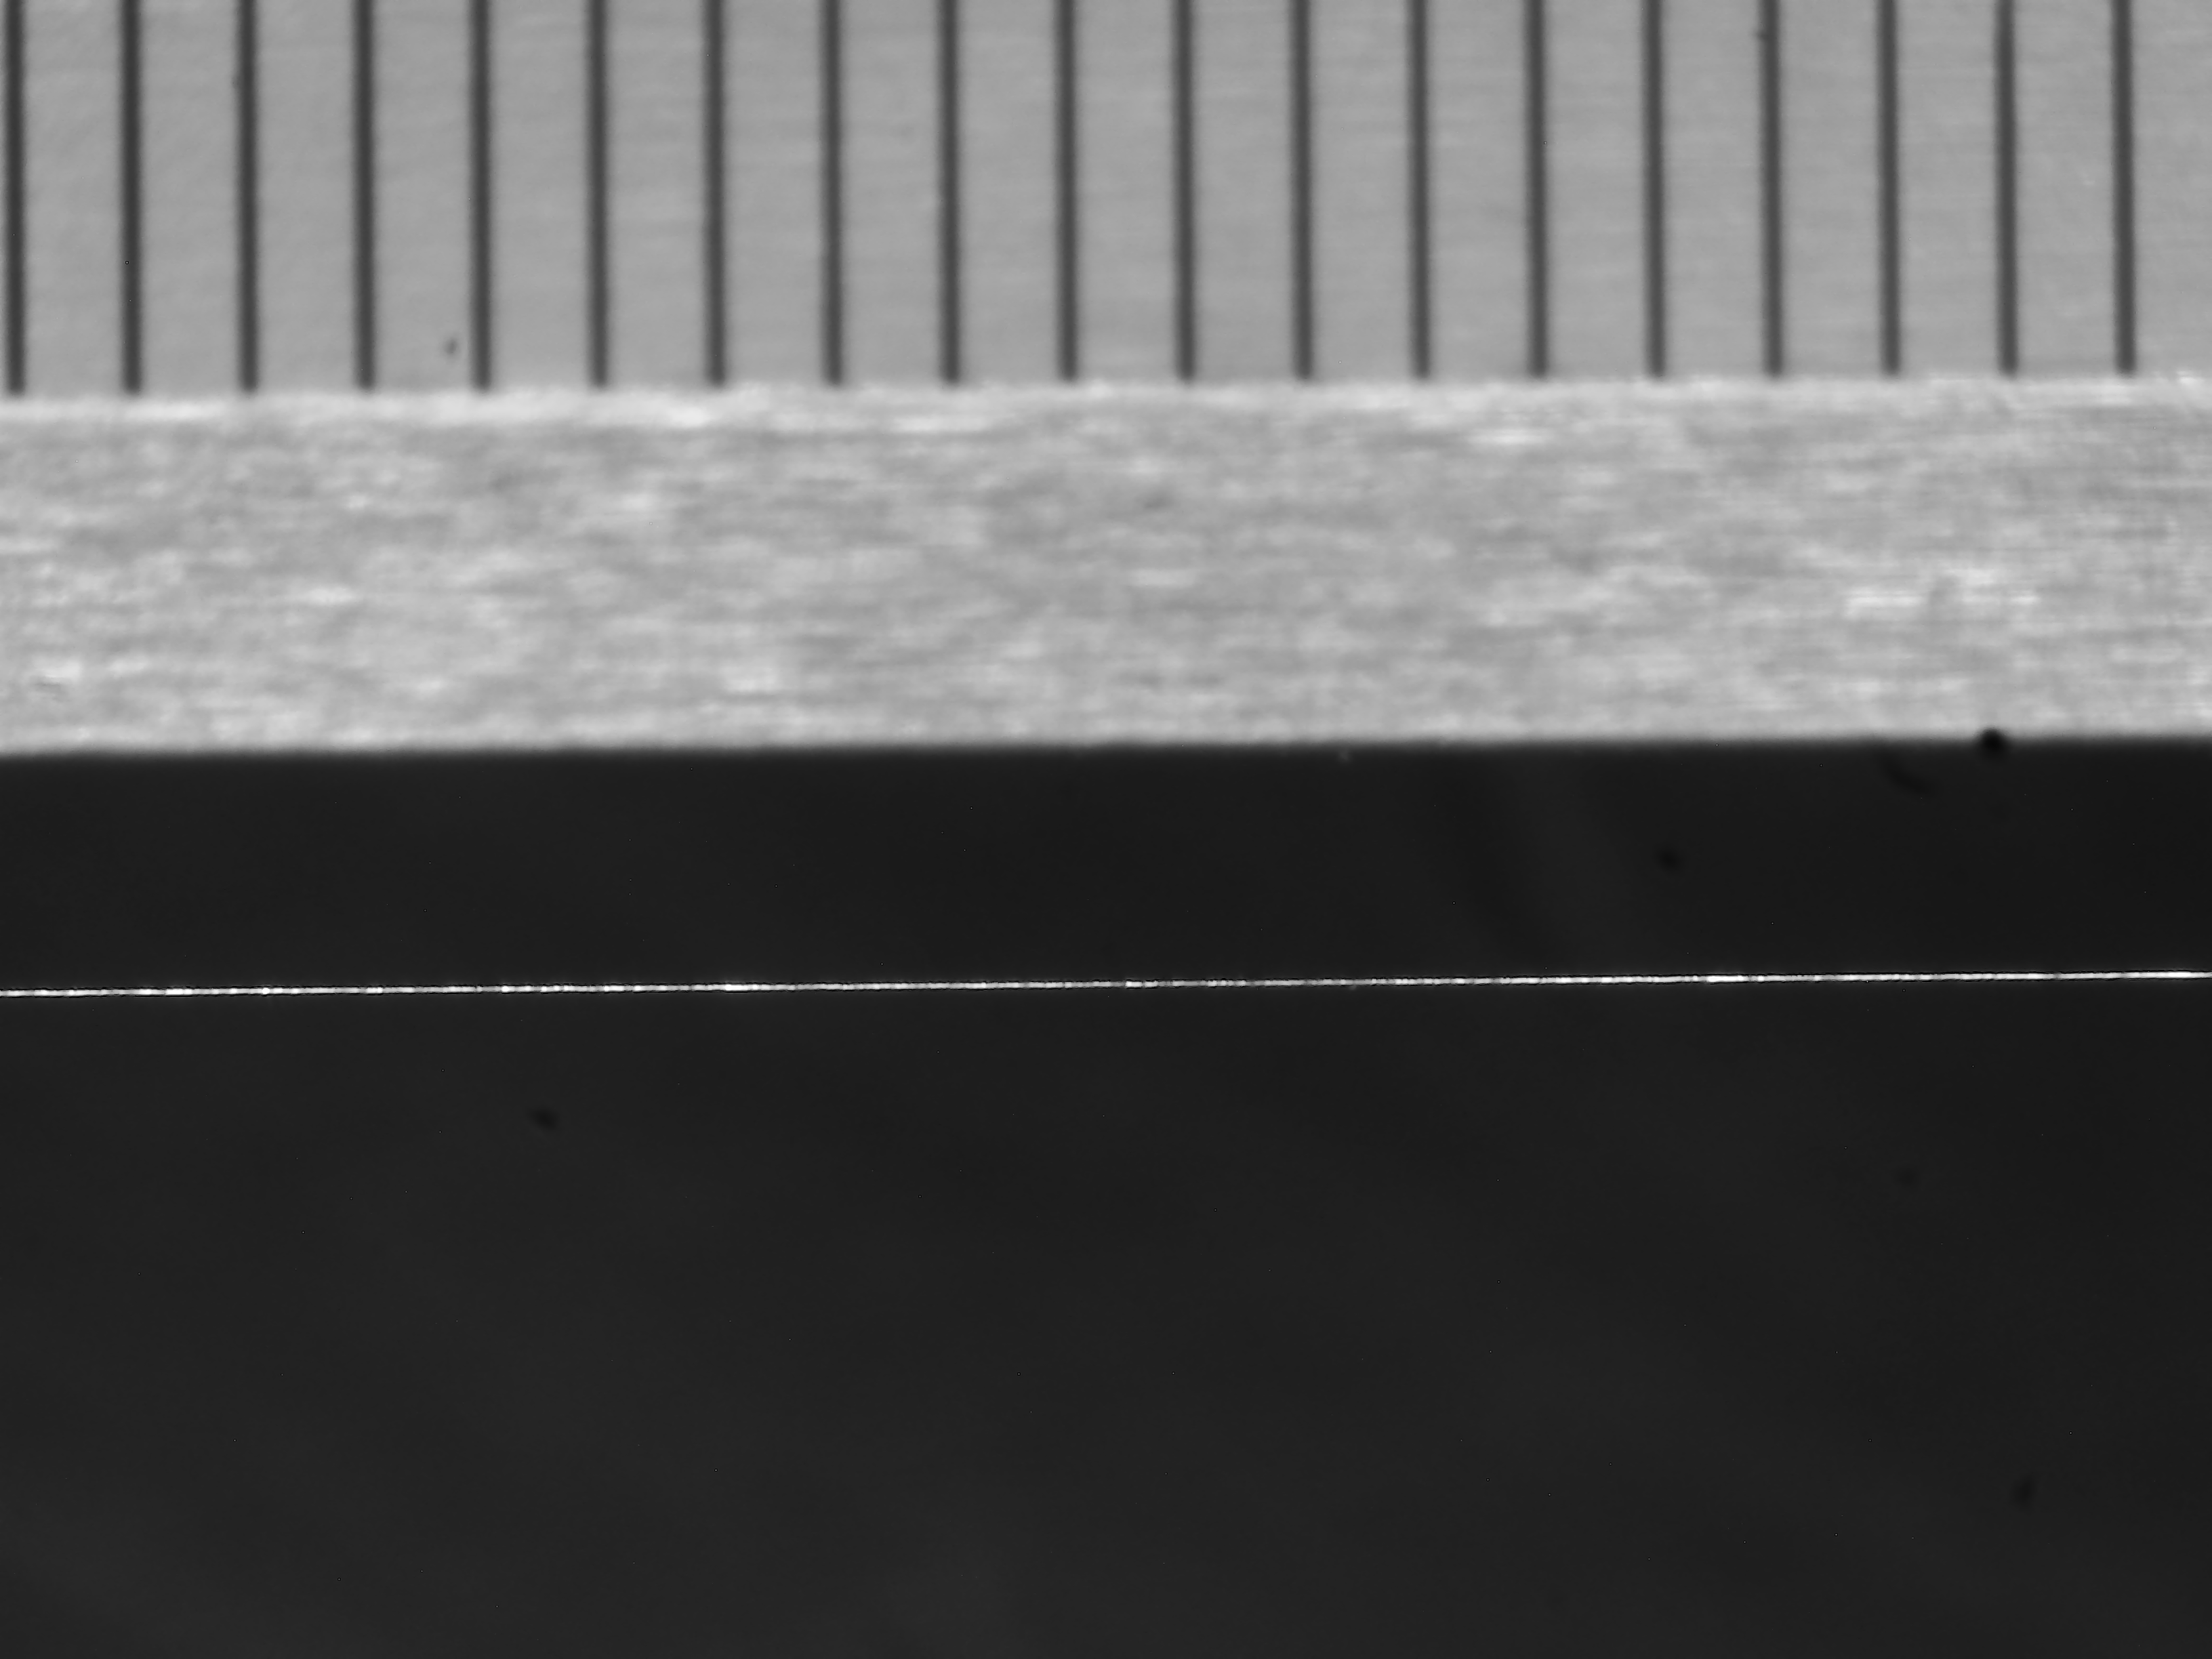
\includegraphics[width=0.7\textwidth]{wiresag/20241217_UHF_3_wire2_x467_gray.png}
    \caption{撮影されたストレートエッジとワイヤーの写真の例}
    \label{fig:wiresag_picture}    
\end{figure}

\subsection{スケーラのfitting}
図\ref{fig:wiresag_scaler_target}、図\ref{fig:wiresag_scaler_brightness}に
$y_{\mathrm{pix}}=\SI{200}{pixel}$ における輝度を示す。
図\ref{fig:wiresag_scaler_brightness}では、横軸を $\SI{1100}{pixel} \leq x_{\mathrm{pix}} \leq \SI{1700}{pixel}$
に拡大したものを合わせて示している。
スケーラの目盛は黒く塗られており、その間は金属により光を反射しているため、その輝度は目盛上で低く、目盛間で高くなる。
理想的には、この輝度の変化は階段関数的である。
一つの目盛とその周りに対して、その輝度は目盛上で低く $B_{\mathrm{scaler}}^{\mathrm{single}}(x)$ は
\begin{align}
    B_{\mathrm{scaler, ideal}}^{\mathrm{single}}(x) &= -\dfrac{B}{2}\qty[\theta(x-x_{\mathrm{left}})+\theta(x_{\mathrm{right}}-x)] + \mathrm{offset} \\
    \theta(x) &= \begin{cases}
        1 & (x>0) \\
        0 & (x\leq 0)
    \end{cases}
\end{align}
のように表せる。$B$ は輝度の最大値と最小値の差、$x_{\mathrm{left}},\,x_{\mathrm{right}}$ は目盛の左端と右端の位置、$\mathrm{offset}$ は輝度のオフセットである。
しかし、実際には写真のピントにより輝度がぼやけてしまい、図\ref{fig:wiresag_scaler_brightness} のように滑らかに輝度が変化する。
そこで、この階段関数をシグモイド間数に置き換えることでこの輝度の変化をモデル化する。
\begin{align}
    B_{\mathrm{scaler}}^{\mathrm{single}}(x) = \dfrac{B}{2}
\end{align}
\begin{figure}[H]
    \centering
    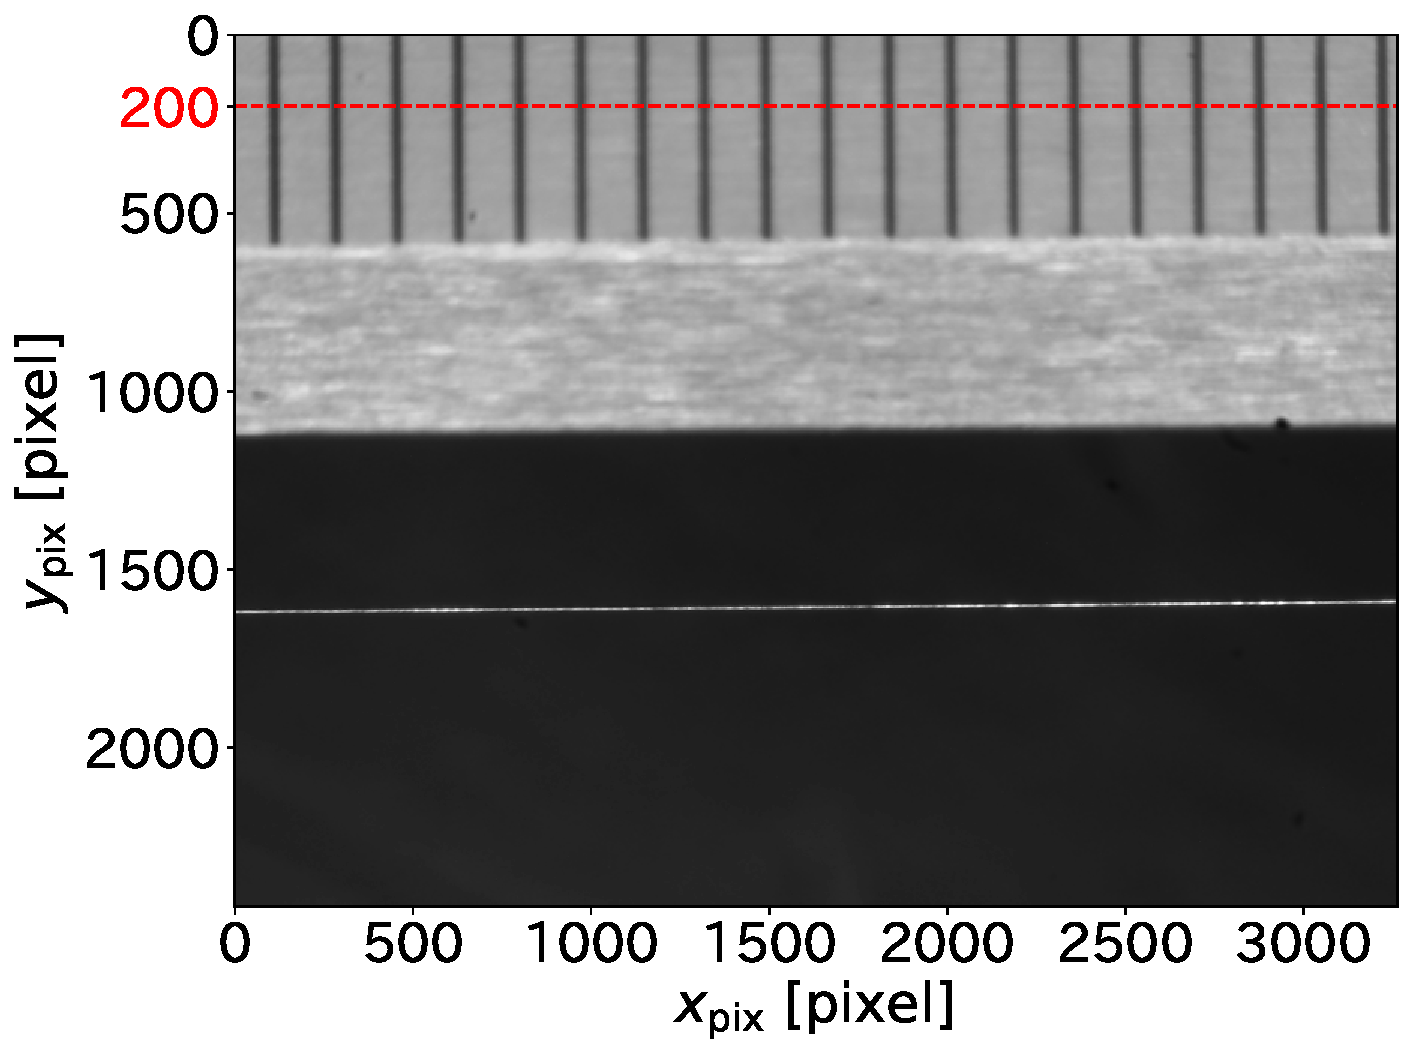
\includegraphics[width=0.7\textwidth]{wiresag/wiresag_scaler_target.pdf}
    \caption{写真中における $y_{\mathrm{pix}}=\SI{200}{pixel}$ の目安}
    \label{fig:wiresag_scaler_target}
\end{figure}
\begin{figure}[H]
    \centering
    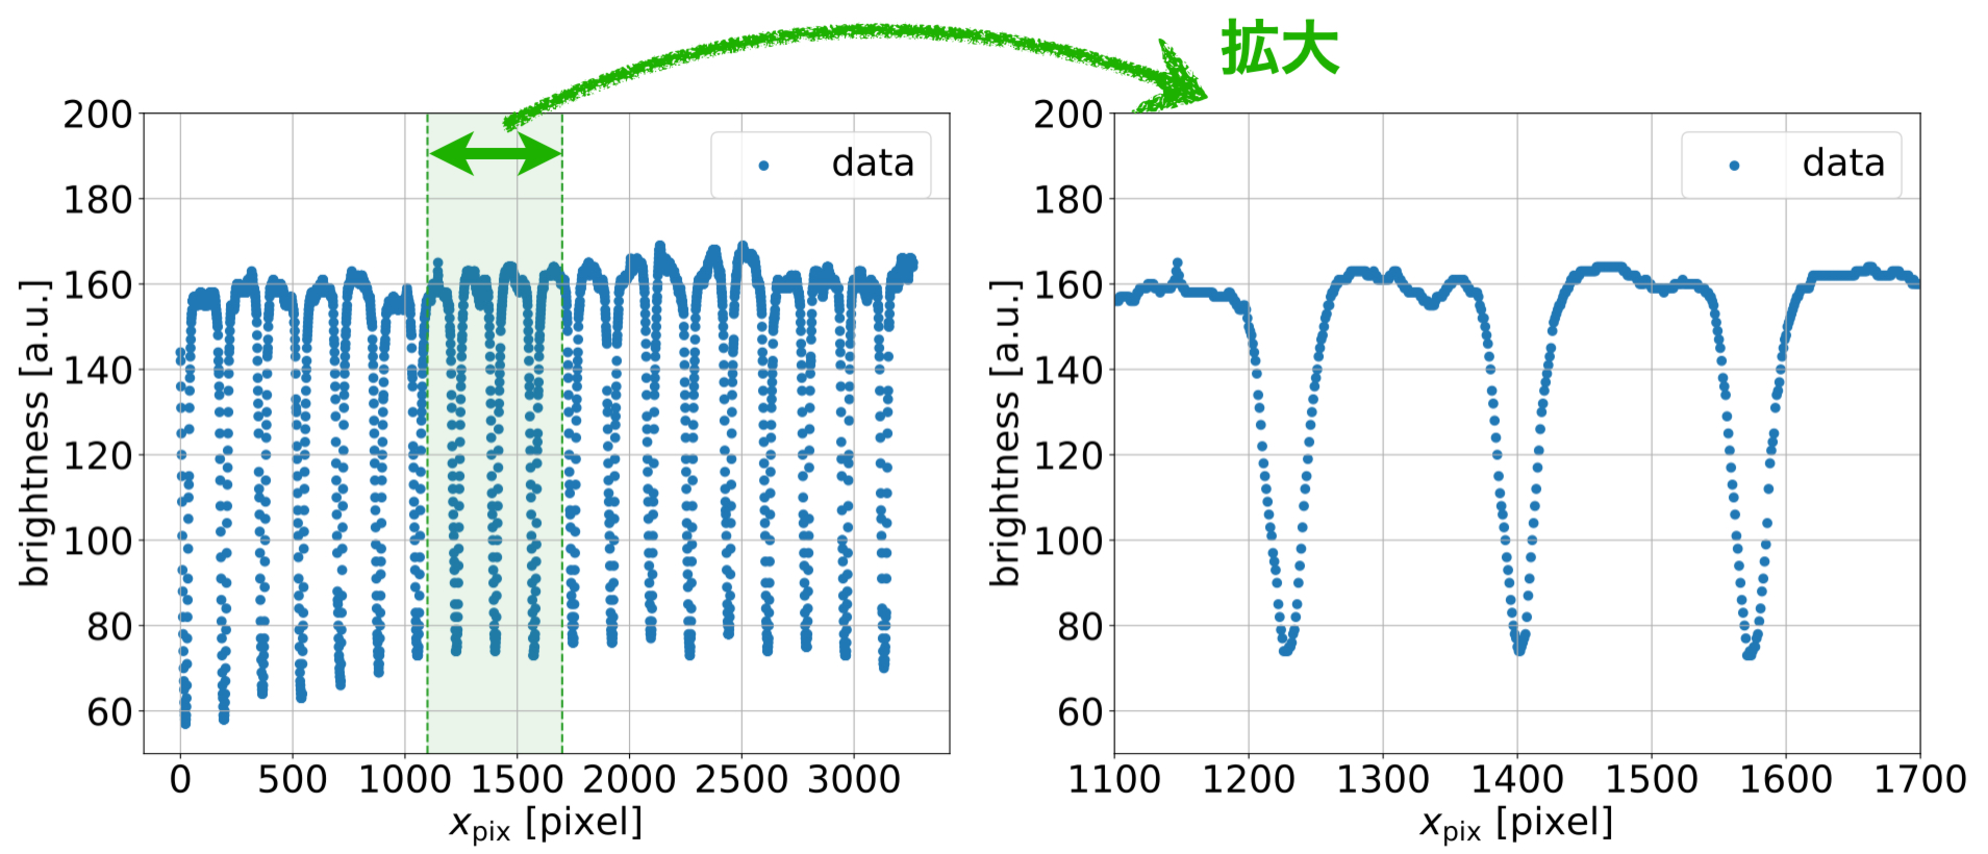
\includegraphics[width=1.0\textwidth]{wiresag/wiresag_scaler_brightness.pdf}
    \caption{$y_{\mathrm{pix}}=\SI{200}{pixel}$ における輝度}
    \label{fig:wiresag_scaler_brightness}
\end{figure}


\subsection{ワイヤーのfitting}
\subsection{ストレートエッジのfitting}
\subsection{画像の回転}
\subsection{カテナリーでのfitting}

\section{開発した評価系の原理検証}
\subsection{評価手法}
\subsection{評価結果とその考察}

\section{スパースワイヤーグリッドのたわみ量の評価}

\end{document}